\documentclass{beamer}
\usefonttheme[stillsansseriflarge]{serif}
%\usecolortheme{spruce}
\usetheme{CambridgeUS}

\makeatletter
\def\ltj@stdmcfont{SourceHanSerifSC}
\def\ltj@stdgtfont{SourceHanSansSC}
\def\ltj@stdyokojfm{eva/{smpl,hgp,nstd}}
\def\ltj@stdtatejfm{eva/{smpl,hgp,nstd,vert}}
\makeatother

\usepackage{luatexja, luatexja-ruby, graphicx, multicol}

\title{USACO竞赛介绍}
\subtitle{Olympiad in Informatics}
\author{黄 京}
\institute{WFLA}
\date{\today}


\begin{document}

\begin{frame}
  \titlepage
\end{frame}

\begin{frame}
  \frametitle{目 次}
  \tableofcontents
\end{frame}

\section{竞赛及相关信息}

\subsection{赛事简介}

\begin{frame}
  \frametitle{信息学竞赛简介}
  \ruby{\textbf{信息学奥林匹克竞赛}}{Olympiad in Informatics}是一门在中学生中广泛开展的学科竞赛,和物理、数学等竞赛性质相同。

  其考察的内容是参赛者运用\ruby{算法}{Algorithm}、\ruby{数据结构}{Data Structure}和数学知识,通过编写计算机程式码解决实际问题的能力。
\end{frame}

\begin{frame}
  \frametitle{竞赛种类列举}
  信息学竞赛种类繁多、仅中国就包括:
  \begin{itemize}
    \item 全国青少年信息学奥林匹克联赛(NOIP)
    \item 全国青少年信息学奥林匹克竞赛(NOI)
    \item 全国青少年信息学奥林匹克竞赛冬令营(WC)
    \item 国际信息学奥林匹克竞赛中国队选拔赛(CTSC)
  \end{itemize}
  国际性的信息学竞赛包括:
  \begin{itemize}
    \item 国际信息学奥林匹克(IOI)
    \item 美国计算机奥林匹克竞赛(USACO)
    \item 日本信息学奥林匹克(JOI)
    \item 亚太地区信息学奥林匹克(APIO)
  \end{itemize}
\end{frame}

\subsection{USACO简介}

\begin{frame}
  \frametitle{USACO相关信息}
  \ruby{\textbf{美国计算机奥林匹克竞赛}}{United States of America Computing Olympiad}是一项针对全世界所有的高中信息学竞赛选手的一项竞赛。

  开设目的是为每年夏季举办的国际信息学奥林匹克选拔美国队队员共4名。含金量非常高。

  每年冬季到初春,USACO会每月举办一场网络赛。一场比赛持续3~5小时。
\end{frame}

\begin{frame}
  \frametitle{可用程式设计语言}
  可用程式设计语言为:
  \begin{itemize}
    \item C/C++(标准11、14、20被支持)
    \item Python(标准3.0.4、2.7.6被支持)
    \item Java JVM
    \item Pascal(Open实现被支持)
  \end{itemize}
\end{frame}

\begin{frame}
  \frametitle{语言避坑}
  \centering
  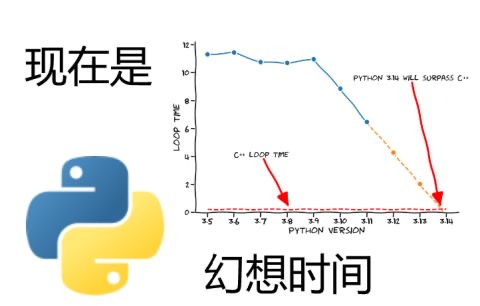
\includegraphics[width=.9\hsize]{pycpp}
\end{frame}

\begin{frame}
  \frametitle{难度评级}
  USACO的比赛分为4档难度。
  \begin{itemize}
    \item \textbf{铜牌组}:适合编程初学者,尤其是那些只会最最基础的算法(如排序、二分查找)的学生;
    \item \textbf{银牌组}:适合开始学习基本的算法技巧(如递归、搜索[DFS、BFS]、贪心算法)和基础数据结构的学生;
    \item \textbf{金牌组}:学生会遇到更复杂的算法(如最短路径、动态规划)和更高级的数据结构(如二叉树、散列表),需要掌握基础的图论、范畴论等数学工具;
    \item \textbf{铂金组}:适合有着扎实算法设计能力的选手,会遇到更加复杂开放的题。
  \end{itemize}
\end{frame}

\section{例题及解析}

\subsection{例题}

\begin{frame}
  \frametitle{Soldier and Number Game}
  \small\parindent=2em
  Two soldiers are playing a game.
  At the beginning first of them chooses a positive integer $n$ and gives it to the second soldier.
  The the second one tries to make maximum possible number of rounds.
  Each round consists of choosing a positive integer $x>1$, such that $n$ is divisible by $x$ and replacing $n$ with $n/x$.
  When $n$ becomes equal to $1$ and there is no more possible valid moves the game is over and the score of the second soldier is equal to the number of rounds he performed.

  To make the game more interesting, first soldier chooses $n$ of form $a!/b!$ for some positive integer $a$ and $b$ ($a \geq b$).
  Here by $k!$ we denote the factorial of $k$ that is defined as a product of all positive integers not larger than $k$.

  What is the maximum possible score of the second soldier?

  The first line of input consists of single integer $t$ ($1 \leq t \leq 1,000,000$) denoting number of games soldiers play.
  Then follow $t$ lines, each contains pairs of integers $a$ and $b$ ($1 \leq b \leq a \leq 5,000,000$) defining the value of $n$ for a game.
\end{frame}

\subsection{题解}

\begin{frame}
  \frametitle{思路(前半)}
  该问题本质即$\prod^a_{i = b + 1} i$每次除以一个因数,最多除几次才为$1$。

  想来要尽可能多得除掉因数,那么除掉的都应是素因数:合因数可用素因数的倍数表示、不好。
\end{frame}

\begin{frame}[fragile]
  \frametitle{埃拉托斯特尼筛法}
  如果每一次对数组的操作花费1个单位时间,则时间复杂度为:
  $$
    O \left( \sum^{\pi(n)}_{k=1} \frac{n}{p_k} \right) =
    O \left( n \sum^{\pi(n)}_{k=1} \frac{1}{p_k} \right).
  $$
  其中$p_k$表示第$k$小的素数,$\pi(n)$表示小于等于$n$的素数个数。
  $\sum^{\pi(n)}_{k=1}$表示第一层\verb|for|循环,其中累加上界$\pi(n)$为\verb|if (prime[i])|进入\verb|true|分支的次数;$\frac{n}{p_k}$表示第二层\verb|for|循环的执行次数。

  根据Mertens第二定理,存在常数$B_1$使得:
  $$
    \sum^{\pi(n)}_{k=1} \frac{1}{p_k} = \log \log n + B_1 + O \left( \frac{1}{\log n} \right).
  $$
  所以该筛法的时间复杂度为$O(n \log \log n)$。
\end{frame}

\begin{frame}[fragile]
  \frametitle{线性筛法}
  埃氏筛法仍有优化空间,它会将一个合数重复多次标记。让每个合数都只被标记一次,那么时间复杂度就可以降到$O(n)$了。

  又称欧拉筛法。

  此题情境中,筛的时候\verb|f[prime[j] * i] = f[i] + 1|即可。原理是除以最小素因子后递推。

  此时得到的是$e \in (a,b]$且$e \in \mathbb{N}$的数组中每个元素可被分解为的(最小)素数(的个数)。
\end{frame}

\begin{frame}
  \frametitle{前缀和}
  前缀和可以简单理解为「数列的前$n$项的和」,是一种重要的预处理方式,能大大降低查询的时间复杂度。

  本题给定的是乘积。显然所求答案为线性筛输出数组的前缀和后数组的某一索引的量。而此时前缀和的递推式为:
  $$
    r(i) = \sum^a_{i = b + 1} f(i-1) + f(i).
  $$
\end{frame}

\begin{frame}[fragile]
  \frametitle{我的C艹实现}
  \tiny
  \begin{multicols}{2}
  \begin{verbatim}
# include <iostream>

const int NLIM = 5e6;
long long prime[NLIM + 3] = {0};
long long prjit[NLIM + 3] = {0};
long long cache[NLIM + 3] = {0};
int prptr = 0;

using namespace std;

inline void factor(int lim)
{
  for (long long i = 2; i <= lim; ++i) {
    if (!prime[i]) {
      prjit[prptr++] = i;
      cache[i] = 1;
    }
    for (int n = 0; n < prptr; ++n) {
      if (i * prjit[n] > lim) break;
      prime[i * prjit[n]] = 1;
      cache[i * prjit[n]] = cache[i] + 1;
      if (i % prjit[n] == 0) break;
    }
  }
}

inline void catjit(int bdr)
{
  for (int x = 1; x <= bdr; ++x)
    cache[x] = cache[x - 1] + cache[x];
}

int main()
{
  ios::sync_with_stdio(false);
  cin.tie(nullptr);

  factor(NLIM + 1);
  catjit(NLIM);

  int t = 0;
  cin >> t;
  while (t--) {
    int a, b;
    cin >> a >> b;
    cout << cache[a] - cache[b] << "\n";
  }

  return 0;
}
  \end{verbatim}
  \end{multicols}
\end{frame}

\begin{frame}
  \frametitle{AC}
  \centering
  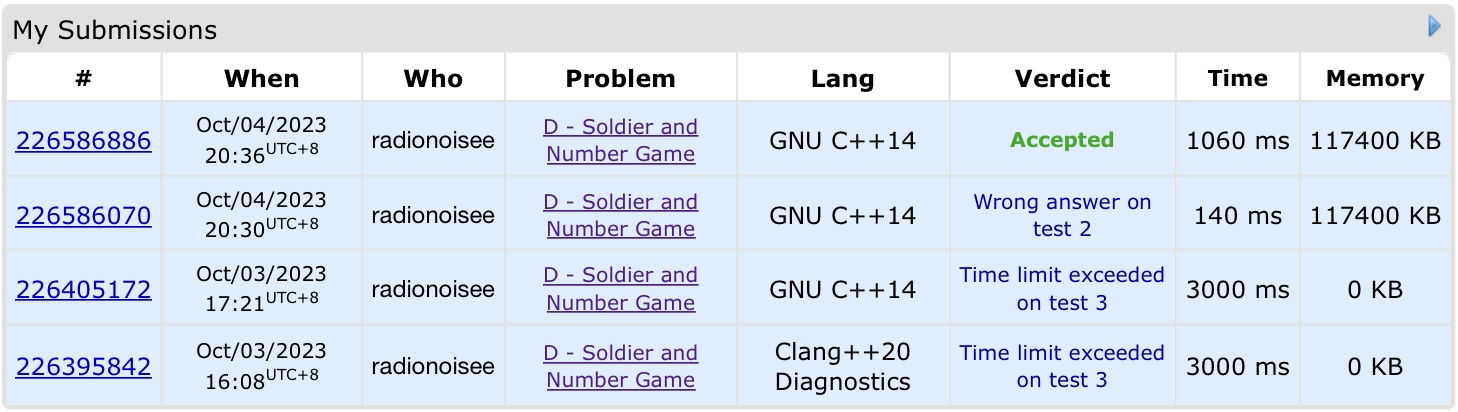
\includegraphics[width=.9\hsize]{smhist}
\end{frame}

\section{终}

\subsection{学习资料}

\begin{frame}
  \frametitle{训练网站}
  \centering
  
\includegraphics[width=.9\hsize]{codeforces}
\end{frame}

\subsection{分发许可}

\begin{frame}
  \frametitle{没 了}
  PDF generated by Lua\TeX.

  Typeset using the \textsf{Beamer} document class with theme \texttt{CambridgeUS}.

  Licensed under Creative Common 1.0 Universal.

  Figures are all extracted from the \texttt{codeforces} forum, which can be redistributed under the terms of this General Public License.
\end{frame}

\end{document}
